\chapter{Vorbereitung zur Umsetzung von Avoidance}\label{chap:intro_avoidance}

Um die Avoidance-Software umzusetzen, wird diese vorher in verschiedenen Modi erprobt. Dazu zählt eine Simulation. Aus dieser können die Strukturen zum Einsatz mit realer Hardware übernommen werden. Als Zwischenschritt wird die \gls{hil}-Simulation aus dem vorhergehenden Projektteil überarbeitet.

\section{Avoidance als Simulation in Software}\label{chap:sim_gazebo}
Das Kapitel spaltet sich auf in die Beschreibung und nachfolgend die programmiertechnischen Schritte zur Umsetzung.

\subsection*{Beschreibung der Umsetzung von Avoidance}
Das Avoidance-Modul arbeitet eng mit der Simulationssoftware \enquote{Gazebo} zusammen. In der Dokumentation \cite{dronecodestiftungObstacleDetectionAvoidance2023} ist die Simulation umfangreich dokumentiert, die Umsetzung des Projektes auf reale Hardware jedoch kurz gehalten.\\
Ein vollständiges Linux Ubuntu 20.04 wird benötigt, um die Software per Simulation verwenden zu können. Die Installation beinhaltet eine komplette \acrshort{ros}-Distribution mit graphischen Tools. Mithilfe mehrerer, sich gegenseitig aufrufenden, \enquote{Launch-Files} wird die Simulation instrumentiert und, aufeinander abgestimmt, gestartet. Ohne weiteres Zutun muss nur das Hauptscript zur jeweiligen Simulation aufgerufen werden. Folgend aufgelistet die vier primären Software Bestandteile:
\begin{description}
    \item[Simulator:] \textit{Gazebo}, erzeugt virtuelle Umgebung in der sich eine simulierte Drohne befindet, kann direkt mit dem Flugcontroller kommunizieren
    \item[Flugcontroller:] PX4-Flightstack, Software zur Steuerung einer Drohne, ohne echte Hardware wird ein Flugcontroller simuliert der eine Konsole und Netzwerkanbindungspunkte (via \acrshort{mav}) bereitstellt
    \item[mavros:] \acrshort{mav}-zu-\acrshort{ros}-Übersetzung, siehe \cite[Kapitel 5.2]{markusreinErweiterungBestehenderDrohnen2023}
    \item[Avoidance:] Je nach gewähltem Programm wird der \textit{Local Planner}, \textit{Global Planner}, oder \textit{Safe Landing Planner} gestartet. In diesem Projekt wird der \textit{Local Planner} erprobt.
\end{description}
Zusätzliche Programme, die beim Ausführen des \textit{Local Planner} gestartet werden, sind:
\begin{description}
    \item[rqt-reconfigure:] Feineinstellungen zum Algorithmus \textit{Local Planner} (bspw. bevorzugte Richtungskorrektur, minimale Größe erkannter Hindernisse)
    \item[rviz:] Visualisierung der Drohne im 3-Dimensionalen Raum, dargestellt wird Position der Drohne, ihres Ursprungs, Zielposition, geplante Flugroute, Punktwolkendarstellung von Hindernis, eventuell Blaupause von Hindernis (Abhängig von gewählter Umgebung)
\end{description}
Für die Untersuchung der gegebenen Situation wird zusätzliche Software verwendet:
\begin{description}
    \item[topic-explorer:] Detaillierte Informationen zu Nachrichten im \acrshort{ros}-Umfeld
    \item[tftree:] Verknüpfungen im Transformationsbaum zur Bestimmung der Position der Drohne und derer Peripherie im Bezug zum Ursprung 
\end{description}

Die Interaktion der Bestandteile ist in Abbildung \ref{fig:system_sim_origin} noch einmal dargestellt. Auf rechter Seite gezeichnet sind die Bestandteile in der \enquote{\acrshort{ros}-Umgebung}, welche in die Endanwendung übernommen werden können. Die vollen Aufgaben des Simulators wurden eingekürzt, sie sind zu lesen in \cref{chap:intro_simulation} und \cite[Kapitel 3.4.1]{markusreinErweiterungBestehenderDrohnen2023}. Zusätzlich stellt der Simulator Kamerabilder bereit, je nach gewähltem Modus direkt Tiefenbilder oder Stereobilder, welche weiter verarbeitet werden müssen. 
\begin{figure}[!ht]
    \centering
    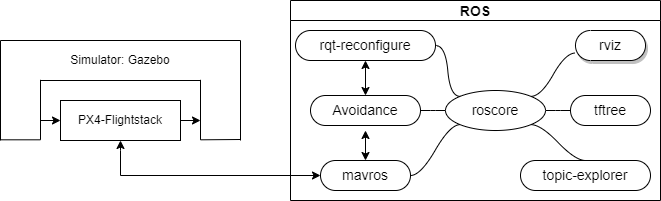
\includegraphics[width=\linewidth]{images/simulation_ros.drawio.png}
    \caption[Systemaufbau der Simulation von Avoidance als Software-Simulation]{Systemaufbau der Simulation von Avoidance als Software-Simulatio: Links Simulator (Gazebo) und Flugcontroller (reine Software), Rechts Bestandteile des \acrshort{ros}}
    \label{fig:system_sim_origin}
\end{figure}

Eine erste Überprüfung des Algorithmus wird die Simulation wie in der Anleitung\footnote{\url{https://github.com/PX4/PX4-Avoidance}\cite{dronecodestiftungObstacleDetectionAvoidance2023}} beschrieben durchgeführt. Einige Paramameter wurden zur besseren Übersichtlichkeit angepasst, sodass:
\begin{itemize}
    \item \textit{Gazebo} mit graphischer Oberfläche startet
    \item Die korrekte Punktwolken-Topic vom \textit{Local Planner} abonniert wird
    \item Die Punktwolke der Kamerabilder noch einmal gefiltert wird
\end{itemize} 

Die Anfangsbedingungen der Simulation sind eine vor Bäumen stehende Drohne. Das Bild aus der Simulation ist abgedruckt im Anhang unter \ref{fig:sim_gazebo}. Von der Drohne werden 2 virtuelle Kamerabilder erzeugt, aus welchen eine Punktwolke gebildet wird. Die Punktwolke ist in Bild \ref{fig:sim_gazebo_stereo} links dargestellt. Der Algorithmus zur Erzeugung der Punktwolke ist anfällig für Rauschen verursacht durch minimale Bewegungen in den Kamerabildern, sodass im Bild Artefakte enthalten sind. Deshalb wurde die Punktwolke noch einmal mit einem VoxelGrid\footnote{\url{http://wiki.ros.org/pcl_ros/Tutorials/VoxelGrid\%20filtering}\cite{openroboticsDocumentationROSWiki}} gefiltert, abgebildet in \ref{fig:sim_gazebo_stereo} rechts. Für die Verwendung der Punktwolke mit Avoidance macht das Filtern keine Auswirkung, der \textit{Local Planner} kommt auch mit den ursrpünglichen Daten der Punktwolke zurecht.

\begin{figure}[!ht]
    \centering
    \subfloat[][Erzeugte Punktwolke]{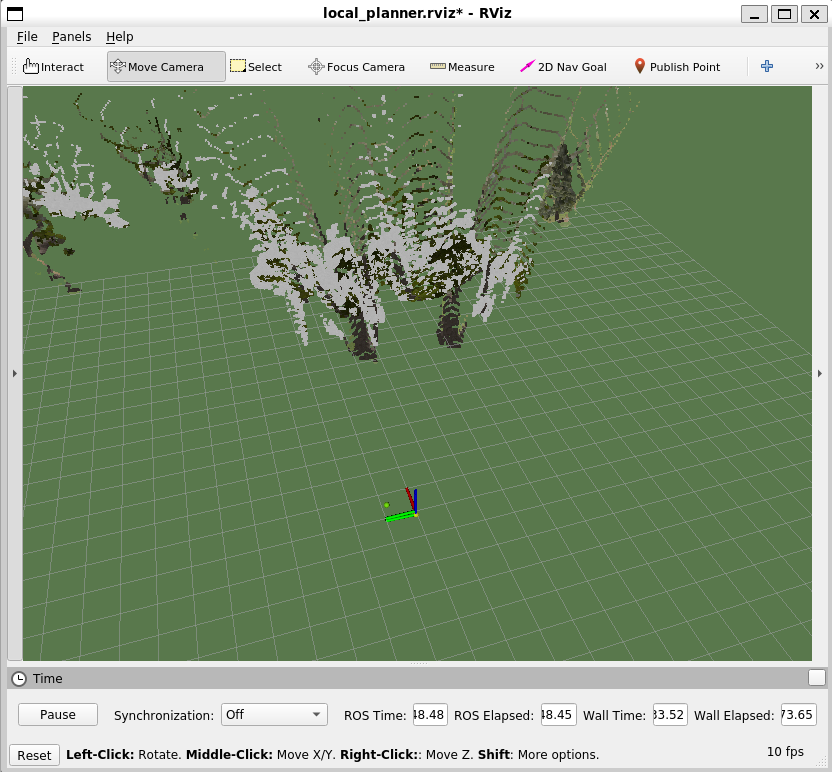
\includegraphics[width=0.4\textwidth]{images/sim_gazebo_points_stereo.png}}\hfill
    \subfloat[][Erzeugte Punktwolke, gefiltert]{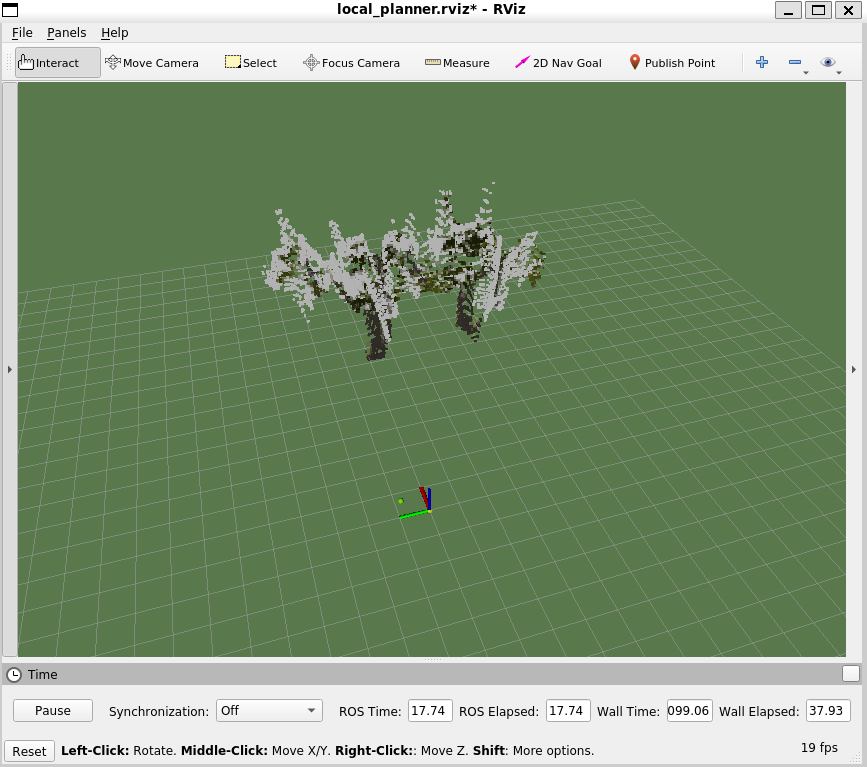
\includegraphics[width=0.4\textwidth]{images/sim_gazebo_points_stereo_voxel.png}}\hfill
    \caption[Punktwolkendarstellung in \textit{rviz}]{Punktwolkendarstellung in \textit{rviz} generiert aus simulierten Bildern}
    \label{fig:sim_gazebo_stereo}
\end{figure}

Zuletzt ist der Transformationsbaum in Bild \ref{fig:sim_gazebo_tftree} abgedruckt. Eine Transformation ist notwendig, um die Position von Objekten (bspw. der Drohne im Raum, Kameras an der Drohne) relativ zu ihrem Bezugspunkt/ Ursprung darzustellen. Die Position der Drohne wird gekennzeichnet durch den Knoten \enquote{fcu} und ist relativ zum Knoten \enquote{local\_origin}. Um alle bekannten Punkte im Raum anpeilen zu können (von einem bekannten Punkt aus), sollten alle Knoten miteinander verknüpft sein. Jedoch besteht der Transformationsbaum hier aus 4 einzelnen Strängen. Dies ist der Konfiguration von \textit{mavros} geschuldet, die wiederrum in \textit{Avoidance} integriert ist. Die Themen \enquote{map} und \enquote{odom} werden von \textit{mavros} zur Navigation genutzt. Die Transformation \enquote{base\_link} wurde in einer neueren Version von \textit{mavros} eingeführt und soll den Mittelpunkt eines Roboters darstellen, wird aber im Projekt nicht genutzt\footnote{\url{https://www.ros.org/reps/rep-0105.html\#base-link}}. Sowohl \textit{mavros} als auch \textit{Avoidance} können mit dem bestehenden Transformationsbaum arbeiten. Wird ein neues Objekt (bspw. Darstellung einer Punktwolke) im Koordinatensystem 
erzeugt, muss auch eine entsprechende Transformation angelegt werden. Für die Tiefenbilder kommt hier das Thema \enquote{camera\_link}, relativ zur Position der Drohne, zum Einsatz.
\begin{figure}[!ht]
    \centering
    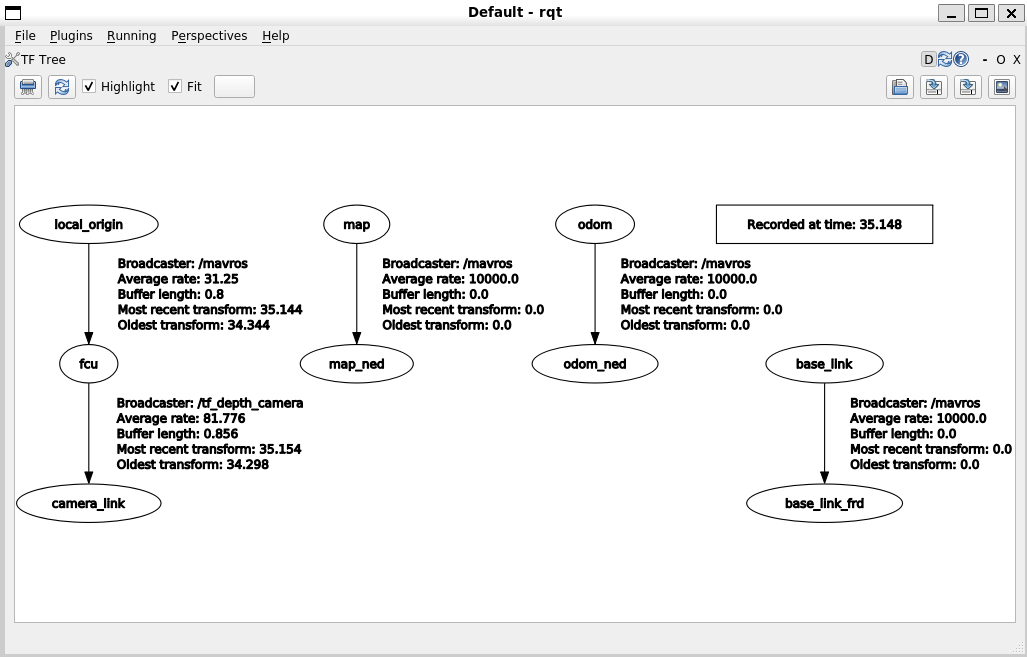
\includegraphics[width=\linewidth]{images/sim_gazebo_tftree.png}
    \caption{Transformationsbaum tftree bei Simulation von \textit{Local Planner}}
    \label{fig:sim_gazebo_tftree}
\end{figure}

\subsection*{Programmierung der Umsetzung von Avoidance}
Im GitHub\cite{dronecodestiftungObstacleDetectionAvoidance2023} ist eine Anleitung zur Installtation von \textit{Avoidance} gegeben. Diese sieht nicht vor in einem Container betrieben zu werden, auch ist die Performance meist nicht ausreichend. Stattdessen wird ein separater Computer benötigt. Im Zweifallsfall funktioniert \textit{Avoidance} doch auch mit den in GitHub bereitgestellten Containern. Es müssen Pakete mit graphischen Anwendungen (bspw. \textit{rviz}, \textit{rqt-reconfigure}) jedoch noch manuell installiert werden, wie in den Dockerfiles von \cite[Kapitel 5]{markusreinErweiterungBestehenderDrohnen2023}\footnote{siehe \url{https://github.com/aur20/T3000-autonomous_drone/tree/airsim_avoidance}} gezeigt.

Anschließend muss der PX4-Flightstack\footnote{https://github.com/PX4/avoidance.git} heruntergeladen werden (bisher im ersten Teil der Arbeit umgangen). Es sind weitere Schritte notwendig, um die Umgebungsvariablen für \textit{Gazebo} und diesen zu setzen. Im Rahmen dieser Arbeit wurden die Schritte als Script zusammengefasst, abgedruckt in Listing \ref{listing:setup_gazebo.sh}. Das Script muss aus dem Verzeichnis \textit{~/catkin\_ws/} ausgeführt werden und der PX4-Flightstack muss sich im Verzeichnis \textit{~/catkin\_ws/src/PX4-Autopilot} befinden.

\section{Avoidance als Simulation mit Hardware}
Als nächste Stufe der Simulation kommt der Simulator \enquote{AirSim} von Microsoft zum Einsatz. Mit \textit{AirSim} stehen die gleichen Möglichkeiten zur Simulation wie mit \textit{Gazebo} zur Verfügung. Allerdings, kann \textit{AirSim} für das Projekt nur mit einem Windows PC zum verwendet werden. Dadurch ergeben sich Beschränkungen, wodurch \textit{AirSim} keine Verbindung zum simulierten Flugcontroller aufbauen kann. Jedoch kann der reale Flugcontroller wie in \cite[Kapitel 5]{markusreinErweiterungBestehenderDrohnen2023} als \gls{hil}-Simulation betrieben werden. Die Veränderungen im Aufbau für die Simulation sind in Bild \ref{fig:system_sim_airsim} rot markiert, die Funktionen der Bestandteile bleiben die gleichen wie in \cref{chap:sim_gazebo}. Hinzu kommt der Bordcomputer, der eine netzwerkgebundene Kommunikation mit dem Flugcontroller erlaubt und der Knoten \enquote{AirSim-Node}, durch den Bilder aus der Simulation ausgelesen werden können. Dabei entfällt das Zusammenfügen zweier Stereobilder, denn die Simulation liefert direkte Tiefenbilder.

\begin{figure}[!ht]
    \centering
    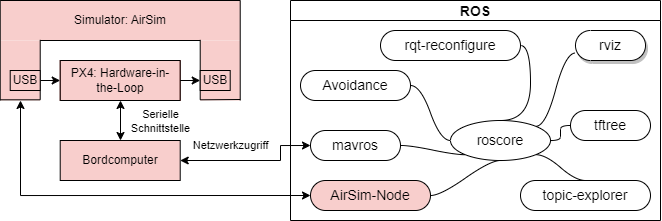
\includegraphics[width=\linewidth]{images/simulation_ros-Page-2.drawio.png}
    \caption[Systemaufbau der Simulation von Avoidance als \gls{hil}-Simulation]{Systemaufbau der Simulation von Avoidance als \gls{hil}-Simulation: Links Simulator (AirSim) und Flugcontroller (\gls{hil}), Rechts Bestandteile des \acrshort{ros}}
    \label{fig:system_sim_airsim}
\end{figure}

Zur Änderung der Funktionalität werden die \textit{Launch-Files} und \enquote{airsim\_ros\_pkgs} (Bibliothek zur Drohnensteuerung im \textit{AirSim}-Simulator) nacheinander angepasst:
\begin{enumerate}
    \item \textit{local\_planner\_stereo.launch}:
    \begin{itemize}
        \item Umbenannt zu \textit{local\_planner\_hitl\_airsim.launch}
        \item Entfernen der Funktion von Disparitätsbildern, da Anwendung keinen ersichtlichen Zweck erfüllt
        \item Unteraufruf von \textit{avoidance\_hitl\_airsim.launch} anstatt \textit{avoidance\_sitl\_stereo.launch}
    \end{itemize}
    \item \textit{avoidance\_sitl\_stereo.launch}:
    \begin{itemize}
        \item Umbenannt zu \textit{avoidance\_hitl\_airsim.launch}
        \item Entfernen der Stereo-Bildverarbeitung, stattdessen Berechnung der Punktwolkendarstellung durch Aufruf von eigens kompiliertem \textit{depth\_image\_proc} aus Tiefenbild von \textit{AirSim}
        \item Entfernen der Transformation von \enquote{fcu} auf \enquote{camera\_link}, da Transformation von Punktwolkendarstellung noch nicht bekannt
        \item Unteraufruf von \textit{avoidance\_hitl\_airsim\_mavros.launch} anstatt \textit{avoidance\_sitl\_mavros.launch}
    \end{itemize}
    \item \textit{avoidance\_sitl\_mavros.launch}:
    \begin{itemize}
        \item Umbenannt zu \textit{avoidance\_hitl\_airsim\_mavros.launch}
        \item Entfernen Startvorgang des \enquote{PX4 SITL} (Software Simulation des Flugcontrollers)
        \item Ändern des Parameters \enquote{fcu\_url} auf lokale IP-Adresse des Onboard-Computers
        \item Ändern des Parameters \enquote{gcs\_url} auf lokale IP-Adresse des Simulations-PC
        \item Entfernen Startvorgang von \textit{Gazebo}
        \item Einfügen Startvorgang der \enquote{AirSim-Node} (Bestandteil der \textit{airsim\_ros\_pkgs}) zur Darstellung eines simulierten Gefährts, dabei noch wichtige Anpassungen: das erzeugte Tiefenbild muss im Untertopic wie die zugehörige \enquote{camera\_info} vorzufinden sein; der Ursprung aller Ortstransformationen, gennant \enquote{world\_frame\_id} wird entsprechend an \textit{local\_origin} angeknüpft
    \end{itemize}
    \item Einstellungen zu \textit{AirSim}:
    \begin{itemize}
        \item Anlegen eines \enquote{vehicle}, hier eine Drohne \textit{PX4} die über USB mit der realen Hardware verbunden ist
        \item Anlegen einer Kamera innerhalb der Drohne, hier vom Typ \enquote{DepthPlanar}, gennant \enquote{mk1}
    \end{itemize}
    \item Einstellungen zu \textit{airsim\_ros\_pkgs}:
    \begin{itemize}
        \item Aufbau einer Verbindung zum Windows-Rechner mit \textit{AirSim}-Simulator
        \item Anhängen des Transformationsbaum von \textit{AirSim} an Transformationsbaum von \textit{mavros} um Transformation der Punktwolke (aus Kamerabild) zur Drohne zu ermöglichen  
        \item Ausgliedern generierter Tiefenbilder aus Transformationsbaum von \textit{AirSim}
        \item Eingliedern generierter Tiefenbilder in Transformationsbaum von \textit{mavros}, dazu wurde die Punktwolke noch entsprechend transformiert, siehe Bild 
    \end{itemize} 
\end{enumerate}

Als Simulation von \textit{AirSim} wurde die \enquote{Blocks}-Umgebung gewählt, eine einfache Welt mit wenigen Objekten. Die Ausgangssituation ist dargestellt im Anhang unter \ref{fig:sim_airsim}. Dabei steht die Drohne vor einem großen Quader. Rechts vom Quader befindet sich eine Kugel.

Probleme die bei der Durchführung durchlaufen wurden, umfassen unter anderem, dass \textit{AirSim} von einem Koordinatensystem im Format \enquote{ENU} (East-North-Up) als die Interpretation der Welt, in der sich die Drohne befindet, ausgeht. Von \textit{mavros} wird die Drohne hingegen im Format \enquote{NED} (North-East-Down) beschrieben. Somit ist das erfasste Kamerabild nicht vor, sondern rechts der Drohne und steht Kopfüber.

Die weitere Entwicklung wurde an diesem Punkt aufgrund mangelnder Zeit eingestellt. Eine Simulation ist bereits vorhanden und lauffähig, der Zwischenschritt \textit{AirSim} wird übersprungen. Bisherige Entwicklungen sind hinterlegt im GitHub\footnote{\url{https://github.com/aur20/T3000-autonomous_drone/tree/airsim_avoidance}}.
